% Global document settings
\documentclass[10pt]{article}

% Packages
\usepackage{tgtermes}
\usepackage{graphicx}
\usepackage{natbib}
\usepackage{authblk}
\usepackage{array}
\usepackage{colortbl}
\usepackage{tocloft}
\usepackage{xcolor}
\usepackage{siunitx}
\usepackage{setspace}
\usepackage{listings}
\usepackage{caption}
\usepackage[T1]{fontenc}
\usepackage[nottoc]{tocbibind}
\usepackage[breaklinks]{hyperref}
\usepackage[font=small,skip=7pt]{caption}

% Custom colours
\definecolor{codegreen}{rgb}{0,0.6,0}
\definecolor{codegray}{rgb}{0.5,0.5,0.5}
\definecolor{codepurple}{rgb}{0.58,0,0.82}
\definecolor{backcolour}{rgb}{0.95,0.95,0.92}

% Listing styles
\lstdefinestyle{mystyle}{
  backgroundcolor=\color{backcolour},
  commentstyle=\color{codegreen},
  keywordstyle=\color{purple},
  numberstyle=\tiny\color{codegray},
  stringstyle=\color{codepurple},
  basicstyle=\ttfamily\footnotesize,
  breakatwhitespace=false,
  breaklines=true,
  captionpos=b,
  keepspaces=true,
  numbers=left,
  numbersep=5pt,
  showspaces=false,
  showstringspaces=true,
  showtabs=false,
  tabsize=2
  }
  \lstset{style=mystyle}

  % Custom commands
  \renewcommand\cftsecafterpnum{\vskip8pt}
  \renewcommand{\lstlistlistingname}{List of \lstlistingname s}
  \renewcommand{\bibsection}{\section*{Bibliography}}
  \renewcommand{\contentsname}{Table of Contents}
  \renewcommand{\bibsection}{\section{\bibname}}
  \renewcommand{\cftsecleader}{\cftdotfill{\cftdotsep}}

  % Custom settings
  \captionsetup{justification=centering}
  \PassOptionsToPackage{hyphens}{url}
  \urlstyle{same}
  \def\Urlmuskip{0mu}
  \def\UrlBreaks{\do\/\do-}
  \hypersetup{
    colorlinks = true,
    urlcolor = blue,
    linkcolor = black,
    citecolor = black,
  breaklinks=true,
  pdfpagemode=UseOutlines,
  bookmarksopen=true,
  bookmarksopenlevel=2,
  bookmarksnumbered=true
  }

  \title{\textbf{From In Vivo to In Silico:} \\ The Role of Animal Models in Advancing Our Understanding of Brain Diseases}
  \author[ ]{Daniel Burger}
  \affil[ ]{\textbf{King's College London}}
  \affil[ ]{\href{mailto:daniel.burger@kcl.ac.uk}{daniel.burger@kcl.ac.uk}}
  \date{\textit{14. February 2023}}

\begin{document}
\pagenumbering{roman}
\counterwithin{lstlisting}{section}
\counterwithin{figure}{section}
\counterwithin{table}{section}

\maketitle
\thispagestyle{empty}

\begin{sloppypar} % For better line breaks
  \begin{abstract}
    Animal models have played a critical role in advancing our understanding of brain diseases. In this essay, we discuss their advantages and limitations and examine two examples of successful advances in our understanding of brain diseases, including one case where they did not deliver the desired outcomes.

    We then look to the future of neuroscience research, including the potential of using cell cultures and computational models in conjunction with animal models. We conclude by emphasising the ongoing importance of animal models in advancing our understanding of brain diseases.

  \end{abstract}
  \pagebreak

  \pagenumbering{Roman}
  \tableofcontents
  \pagebreak

  \listoffigures
  \listoftables
  \pagebreak


  % Double spacing for feedback
  \doublespacing

  \pagenumbering{arabic}
  \section{Introduction}
  \label{sec:introduction}

  Animal models have been invaluable tools in biomedical research, particularly in the field of neuroscience. Through the use of animal models, it is possible to delve into the complexity of our brains and uncover ways that diseases manifest themselves. In vitro, in vivo, and in silico research are some of the methods utilised in neuroscience research, as shown in \autoref{tab:overview-research-methods}. However, in vivo animal models provide a unique advantage in allowing researchers to study the entire organism in a controlled environment, where many variables can be controlled.

  \vspace{10pt} % Increase vertical spacing before table
  \begin{table}[ht]
    \centering
    \renewcommand{\arraystretch}{1.5}
    \setlength{\tabcolsep}{12pt}
    \resizebox{\linewidth}{!}{%
      \begin{tabular}{|>{\hspace{0pt}}m{0.18\linewidth}|>{\hspace{0pt}}m{0.78\linewidth}|} % adjust column widths
        \hline
        \rowcolor[rgb]{0.961,0.961,0.961} \textbf{Method} & \textbf{Definition}                                                                                                         \\
        \hline
        In vitro                                          & Research conducted using isolated biological components in a controlled environment, such as cell cultures or organoids.    \\
        \hline
        In vivo                                           & Research conducted using living organisms, often using animal models, to study the effects of a treatment or intervention.  \\
        \hline
        In silico                                         & Research conducted using computational models or simulations to predict the effects of interventions on biological systems. \\
        \hline
      \end{tabular}
    }
    \caption{Overview of In Vitro, In Vivo, and In Silico Research Methods.}
    \label{tab:overview-research-methods}
  \end{table}

  The use of animal models is crucial in the study of diseases affecting the human brain. While we cannot use humans in every case due to ethical concerns, animal models allow us to study the progression of diseases in a way that is impossible with human subjects. In addition, researchers can use animal models to investigate disease mechanisms at the molecular, cellular, and systemic levels, which is difficult or impossible to do in humans since, for example, the modification of human genomes is not possible due to ethical and safety concerns.

  Animal models have significantly advanced our understanding of many neurological disorders, such as Alzheimer’s, Parkinson’s, and stroke. They allow us to gain insight into the underlying mechanisms of these diseases, which can then lead to new therapies or treatments. For example, studies utilising mouse models have helped researchers better understand the role of genetics in Alzheimer’s disease \citep{holtzman_alzheimers_2011} and Parkinson’s \citep{hernandez_genetics_2016}. Additionally, animal models have been instrumental in providing insight into the effects of substances, such as the effect of prenatal alcohol consumption on the brain \citep{bisen_proteomic_2019}.

  Research with animal models is commonly utilised to assess the safety and effectiveness of potential treatments and drug therapies for neurological diseases, thus reducing the chances of unfavourable outcomes in human trials. This process involves obtaining various types of value from animal models, such as face value, predictive value, and construct value, to assist with translating research findings to humans. Additionally, researchers can now manipulate neuronal networks in model animals using new technologies such as optogenetics and chemogenetics, providing a better understanding of disease pathology.

  However, it is important to note that animal models do have limitations. While they can provide valuable insight into disease mechanisms, they do not always translate perfectly to human disease. Moreover, there are ethical concerns surrounding the use of animals in research, which has led to the development of alternatives such as cell cultures and dish brains.

  In conclusion, animal models have been instrumental in advancing our understanding and treatment of diseases, especially in the field of neuroscience. While they have limitations and ethical considerations, the ability to study the entire organism, generate genetically modified strains, and modify neuronal networks in controlled environments provides researchers with invaluable insight into disease mechanisms. Moreover, with the advent of new technologies and complementary methods, such as computational neuroscience and in vitro approaches, animal models can be combined with other techniques to help solve the mysteries of the human brain.

  \section{Advancements with Animal Models}
  \label{sec:advancements}

  In this chapter, the author discusses two original research papers as listed in \autoref{tab:positive-studies} that illustrate the critical role of animal models in neuroscience research. The first study, “Deep Brain Stimulation of the Rat Subthalamic Nucleus Induced Inhibition of Median Raphe Serotonergic and Dopaminergic Neurotransmission” \citep{kocabicak_deep_2014}, used animal models to examine the effects of subthalamic stimulation on advanced Parkinson’s disease. The results showed that stimulating the subthalamic nucleus in rats with advanced Parkinson’s disease led to improved motor function and a reduction in symptoms related to depression.

  The second study, “Huntington’s disease protein contributes to RNA-mediated gene silencing through association with Argonaute and P bodies,” \citep{savas_huntingtons_2008} used animal models to investigate the underlying mechanisms of Huntington’s disease. The study found a new gene in people with Huntington’s disease that repeats more times than it should, making it unstable. The study also showed that a group of proteins called the Ago family play a crucial role in controlling how genes are silenced through small RNA.

  \vspace{10pt} % Increase vertical spacing before table
  \begin{table}[ht]
    \centering
    \renewcommand{\arraystretch}{1.5}
    \setlength{\tabcolsep}{12pt}
    \resizebox{\linewidth}{!}{%
      \begin{tabular}{|>{\hspace{0pt}}m{0.34\linewidth}|>{\hspace{0pt}}m{0.6\linewidth}|}
        \hline
        \rowcolor[rgb]{0.961,0.961,0.961} \textbf{Study}                                                                                           & \textbf{Main Conclusion}                                                                                                                                                                                                                                                                            \\
        \hline
        “Deep Brain Stimulation of the Rat Subthalamic Nucleus Induced Inhibition of Median Raphe Serotonergic and Dopaminergic Neurotransmission” & Stimulating the subthalamic area in rats with advanced Parkinson’s disease, the rats’ motor function improved and symptoms related to depression decreased. The stimulation was done safely in mice, which allowed researchers to see the effects on the brain without putting humans at risk.      \\
        \hline
        “Huntington’s disease protein contributes to RNA-mediated gene silencing through association with Argonaute and P bodies”                  & A novel gene (Huntingtin) has a repeating pattern of three building blocks that is longer than it should be, which can cause the gene not to work properly. The researchers found that this gene is unstable, meaning it can change and become longer over time, making Huntington’s disease worse. \\
        \hline
      \end{tabular}
    }
    \caption{Two studies showcasing the benefits of animal models: Summary of findings.}
    \label{tab:positive-studies}
  \end{table}


  \subsection{Deep Brain Stimulation for Parkinson’s Disease}
  \label{sec:deep-brain-stimulation}

  The research investigated the effects of subthalamic stimulation on rats diagnosed with advanced Parkinson’s disease through animal models. Rodents were selected as subjects for their favourable attributes, including their small size, short lifespan, and low cost, making them ideal for laboratory experiments involving brain implants such as DBS. Additionally, their physiological similarity to humans makes them a good representation for studying the effects of interventions in humans.

  \begin{figure}[ht]
    \centering
    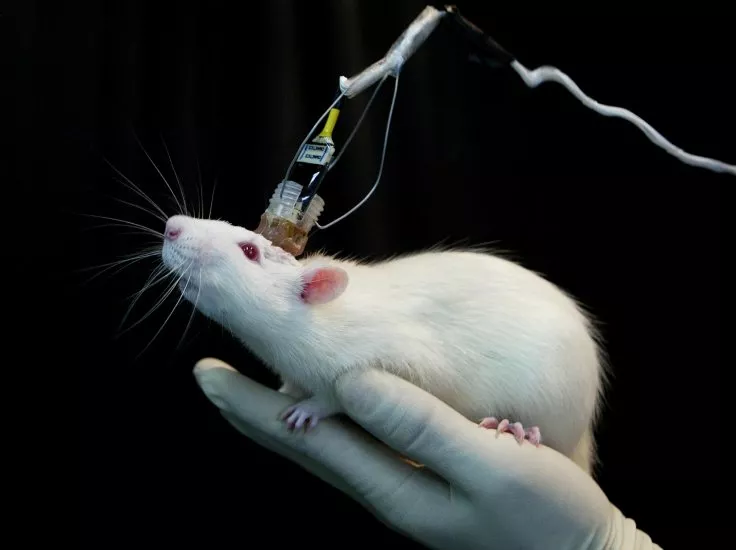
\includegraphics[width=\textwidth]{figures/scientist-deep-brain-stimulation.png}
    \caption[Depiction of a mouse with an electrode implant]{Depiction of a mouse with an electrode implant \citep{sharma_scientists_2017}.}
    \label{fig:dbs-implant}
  \end{figure}

  Animal models, in this case, rats, provide a more realistic portrayal of the effects of an intervention as they allow for the study of the intervention’s impact on a living organism, replicating a more natural environment and providing a closer approximation to human physiology than in vitro methods.

  Twenty male albino Sprague Dawley rats underwent electrode implantation (exemplary depiction in \autoref{fig:dbs-implant}) and stimulation sessions. After the stimulation, the rats’ brains were removed and processed to determine the location of the electrode tips.

  The use of animal models in this research created a safe and controlled environment to study the effects of subthalamic stimulation on the brain, yielding valuable insights and emphasising the critical role that animal models play in neuroscience research.

  \subsection{Gene Silencing in Huntington's Disease}
  \label{sec:huntingtons}

  \begin{figure}[ht]
    \centering
    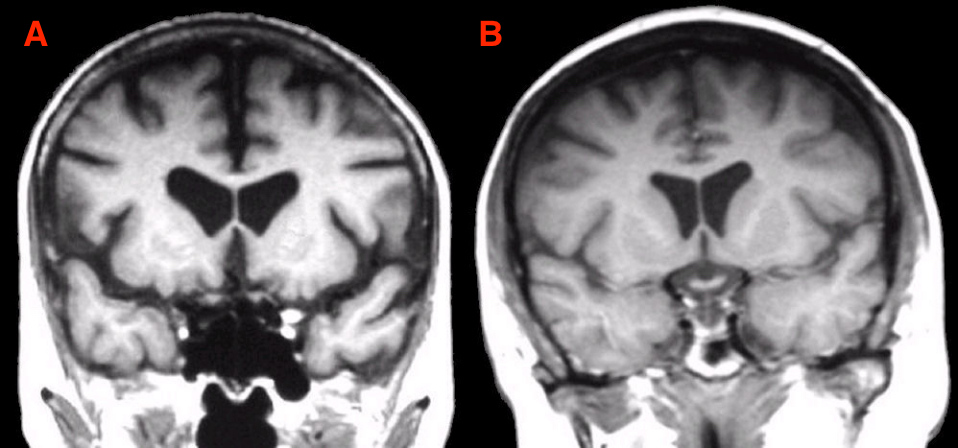
\includegraphics[width=\textwidth]{figures/huntington.jpg}
    \caption[Brain scan of the caudate nucleus in two different conditions, symbol A represents a patient diagnosed with Huntington's disease, while symbol B represents a patient without the condition]{Brain scan of the caudate nucleus in two different conditions, symbol A represents a patient diagnosed with Huntington's disease, while symbol B represents a patient without the condition \citep{c_preston_huntingtons_nodate}.}
    \label{fig:huntingtons}
  \end{figure}


  \section{Shortcomings of Animal Models}
  \label{sec:shortcomings}

  Animal studies have shown that NMDA receptor antagonists can reduce brain damage caused by stroke. However, clinical trials in humans have not been successful in replicating the same results. For example, the drug selfotel, which was effective in animal studies, failed to show a significant clinical benefit in a large human clinical trial.

  Another example is the use of neuroprotective agents for the treatment of traumatic brain injury. Many neuroprotective agents have shown promise in animal studies, but clinical trials in humans have been largely unsuccessful. For example, the drug tirilazad was found to be effective in animal models of traumatic brain injury but did not show a significant clinical benefit in human clinical trials.

  These examples highlight the importance of carefully evaluating the effectiveness of interventions in both animal models and humans and suggest that the translation of findings from animal models to humans is not always straightforward.

  \section{Combination of Different Research Methods}
  \label{sec:discussion}

  \section{Conclusion}
  \label{sec:conclusion}

  \pagebreak
  \bibliographystyle{references/custom-apa}
  \bibliography{references/bibliography}

\end{sloppypar}
\end{document}